\documentclass[12pt,a4paper]{article}
\usepackage[a4paper,top=15mm,bottom=15mm,left=16mm,right=16mm]{geometry}
\usepackage[T1]{fontenc}
\usepackage{amsmath}
\usepackage{amssymb}
\usepackage{array}
\usepackage{tikz}

\pagestyle{empty}
\setlength{\parindent}{0pt}
\setlength{\parskip}{4pt}
\allowdisplaybreaks

% A topic from the revision list, with its "Remember" line from the
% revision guide.
\newcommand{\ptitle}[2]{%
  \par\addvspace{10pt}
  \noindent\rule{\linewidth}{0.8pt}\par\nobreak\vspace{1pt}
  \noindent{\large\bfseries #1}\par\nobreak\vspace{1pt}
  \noindent\textbf{Remember: #2}\par\nobreak\vspace{1pt}
  \noindent\rule{\linewidth}{0.4pt}\par\nobreak\vspace{4pt}}
\newcommand{\wq}[1]{\par\addvspace{6pt}\noindent\textbf{Q#1.}\ }

% \venn{<left set>}{<right set>}{<left only>}{<both>}{<right only>}{<outside>}
\newcommand{\venn}[6]{%
  \begin{tikzpicture}[x=1mm,y=1mm]
    \draw (0,0) rectangle (66,34);
    \node[anchor=north west] at (0,34) {$\xi$};
    \draw (24,17) circle (13.5);
    \draw (42,17) circle (13.5);
    \node at (10,30) {$#1$};
    \node at (56,30) {$#2$};
    \node[align=center] at (17.5,17) {#3};
    \node[align=center] at (33,17) {#4};
    \node[align=center] at (48.5,17) {#5};
    #6
  \end{tikzpicture}}

\begin{document}

\begin{center}
{\Large\bfseries Probability}\\[3pt]
{\large Revision questions: worked solutions}
\end{center}

% ----------------------------------------------------------------
\ptitle{Writing probabilities as fractions, decimals and percentages}{Always between 0 and 1: 0 is impossible, 1 is certain.}

\wq{1} There are $4+6+10=20$ sweets, and 4 of them are green.
\[ \text{P(green)}=\frac{\text{number of ways it can happen}}{\text{total number of possible outcomes}}=\frac4{20}=\frac15=0.2=20\% \]

\wq{2} Probability it does not happen $=1-$ probability it does happen:\quad $1-0.12=0.88$

\wq{3} All the outcomes add up to 1:\quad $0.3+0.25+0.15=0.7$, so P(yellow) $=1-0.7=0.3$

% ----------------------------------------------------------------
\ptitle{Listing outcomes systematically}{Fix one, change the other, work in order, systematically.}

\wq{4} Fix the starter, then change the main:
\[ \text{SF, SC}\qquad \text{MF, MC}\qquad \text{PF, PC} \]
That is $3\times2=6$ meals, which checks that none are missing.

\wq{5} (a) Each row fixes spinner A, and each column changes spinner B.

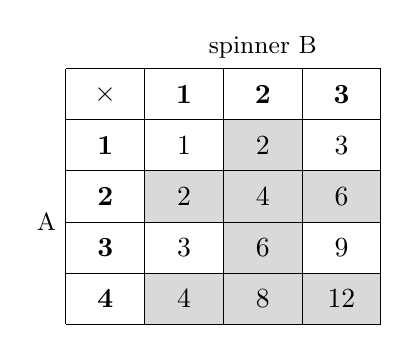
\begin{tikzpicture}[x=10mm,y=6.5mm]
  \foreach \a/\b in {1/2,2/1,2/2,2/3,3/2,4/1,4/2,4/3}{\fill[black!15] (\b,-\a) rectangle ++(1,1);}
  \draw[step={(1,1)}] (0,-4) grid (4,1);
  \node at (0.5,0.5) {$\times$};
  \foreach \b in {1,2,3}{\node at (\b+0.5,0.5) {\textbf{\b}};}
  \foreach \a in {1,...,4}{
    \node at (0.5,-\a+0.5) {\textbf{\a}};
    \foreach \b in {1,2,3}{\pgfmathtruncatemacro{\p}{\a*\b}\node at (\b+0.5,-\a+0.5) {\p};}}
  \node[above] at (2.5,1) {\small spinner B};
  \node[left] at (0,-2) {\small A};
\end{tikzpicture}

(b) 8 of the 12 outcomes are even (shaded), so P(even) $=\dfrac8{12}=\dfrac23$.

% ----------------------------------------------------------------
\ptitle{Expected results}{Probability times the number of goes.}

\wq{6} Expected frequency $=$ probability $\times$ number of trials $=\dfrac12\times300=150$ heads

\wq{7} $0.08\times250=20$ journeys

% ----------------------------------------------------------------
\ptitle{Experimental probability}{More trials, more trust.}

\wq{8} (a) Relative frequency $=\dfrac{\text{number of times it happened}}{\text{total number of trials}}=\dfrac{36}{200}=0.18$

(b) A fair dice gives each score with probability $\frac16$, so in 200 rolls we expect each score about $\frac16\times200\approx33$ times. Every frequency is between 30 and 36, which is close to 33, so the results suggest the dice is fair.

\wq{9} Kai's estimate is better, because he did many more trials.
\[ \text{relative frequency}=\frac{260}{500}=0.52 \]

% ----------------------------------------------------------------
\ptitle{Frequency trees}{Branches add back up to the number before.}

\wq{10} (a) Children: $120-70=50$.\quad Adults with no book: $70-45=25$.\quad Children with no book: $50-20=30$.

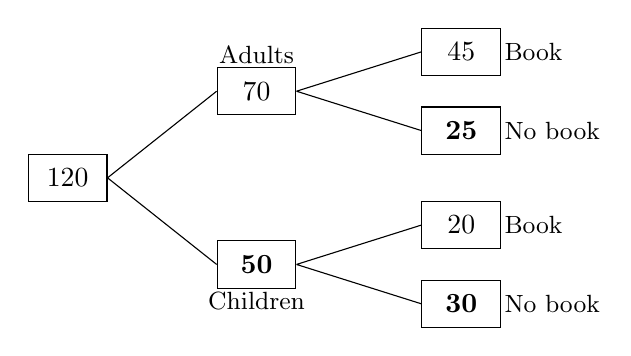
\begin{tikzpicture}[x=1mm,y=1mm,
    box/.style={draw,minimum width=10mm,minimum height=6mm,inner sep=1pt},
    lab/.style={font=\small,inner sep=1pt}]
  \node[box] (r) at (0,0) {120};
  \node[box] (u) at (24,11) {70};
  \node[lab,above] at (u.north) {Adults};
  \node[box] (d) at (24,-11) {\textbf{50}};
  \node[lab,below] at (d.south) {Children};
  \node[box] (uu) at (50,16) {45};
  \node[box] (ud) at (50,6) {\textbf{25}};
  \node[box] (du) at (50,-6) {20};
  \node[box] (dd) at (50,-16) {\textbf{30}};
  \foreach \n in {uu,du}{\node[lab,right] at (\n.east) {Book};}
  \foreach \n in {ud,dd}{\node[lab,right] at (\n.east) {No book};}
  \draw (r.east) -- (u.west) (r.east) -- (d.west);
  \draw (u.east) -- (uu.west) (u.east) -- (ud.west);
  \draw (d.east) -- (du.west) (d.east) -- (dd.west);
\end{tikzpicture}

(b) $45+20=65$ people bought a guidebook, out of 120:\quad P(book) $=\dfrac{65}{120}=\dfrac{13}{24}$

% ----------------------------------------------------------------
\ptitle{Venn diagrams}{Fill the overlap first, then the rest, then outside.}

\wq{11} (a) Overlap: 8.\quad French only: $28-8=20$.\quad Spanish only: $19-8=11$.\quad Outside: $50-20-8-11=11$.

\venn{F}{S}{20}{8}{11}{\node at (60,4) {11};}

(b) P(neither) $=\dfrac{11}{50}$

\wq{12} (a) $A\cap B$ is the overlap: just the number 4.\quad P$(A\cap B)=\dfrac1{15}$

(b) $A\cup B$ is everything inside the circles: 2, 4, 6, 8, 10, 12, 14, 1 and 9.\quad P$(A\cup B)=\dfrac9{15}=\dfrac35$

(c) $A'$ is everything outside circle A: 1, 9, 3, 5, 7, 11, 13 and 15.\quad P$(A')=\dfrac8{15}$

% ----------------------------------------------------------------
\ptitle{Conditional probability with Venn diagrams}{`Given' shrinks your total to just that group.}

\wq{13} (a) Count everything inside the dog circle: $10+21=31$ people.\quad P(dog) $=\dfrac{31}{60}$

(b) Given they own a dog: only look inside the dog circle, which holds 31 people. 10 of them also own a cat.
\[ \text{P(cat)}=\frac{10}{10+21}=\frac{10}{31} \]

\wq{14} Given they study French: only look inside the French circle, which holds $20+8=28$ pupils. 8 of them also study Spanish.
\[ \text{P(Spanish)}=\frac8{28}=\frac27 \]

% ----------------------------------------------------------------
\par\addvspace{10pt}
\noindent\rule{\linewidth}{0.8pt}\par\nobreak\vspace{1pt}
\noindent{\large\bfseries Problem solving}\par\nobreak\vspace{1pt}
\noindent\rule{\linewidth}{0.4pt}\par\nobreak\vspace{4pt}

\wq{15} Try the smallest bag first: 3 red and 5 blue. Adding 2 red gives 5 red and 5 blue, so P(red) $=\frac5{10}=\frac12$. This works, so there were 8 counters at the start.

With algebra: $3k$ red and $5k$ blue.
\[ \frac{3k+2}{8k+2}=\frac12\ \Rightarrow\ 6k+4=8k+2\ \Rightarrow\ k=1 \]

\wq{16} Each section has probability $\frac15=0.2$. P(red) $=0.4$ needs 2 red sections. That leaves 3 sections, and blue has twice as many as green, so 2 blue and 1 green.

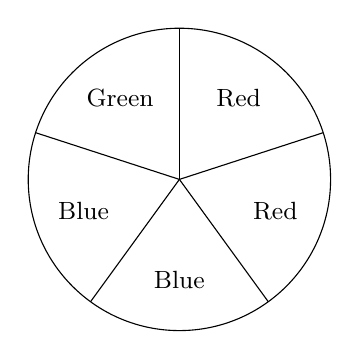
\begin{tikzpicture}[scale=1.6]
  \foreach \i/\c in {0/Red,1/Red,2/Blue,3/Blue,4/Green}{
    \draw (0,0) -- ({90-72*\i}:1.2);
    \node at ({54-72*\i}:0.8) {\small\c};}
  \draw (0,0) circle (1.2);
\end{tikzpicture}

\wq{17} No. With a fair dice, the expected number of 6s in 6 rolls is only $\frac16\times6=1$, so getting no 6s at all is quite likely. Six rolls is far too few to decide. Sam should roll the dice many more times and look at the relative frequency of 6s: more trials, more trust.

\end{document}
